\documentclass{article}
\usepackage{pgfplots}
\usepackage{pgfplotstable}

\begin{document}

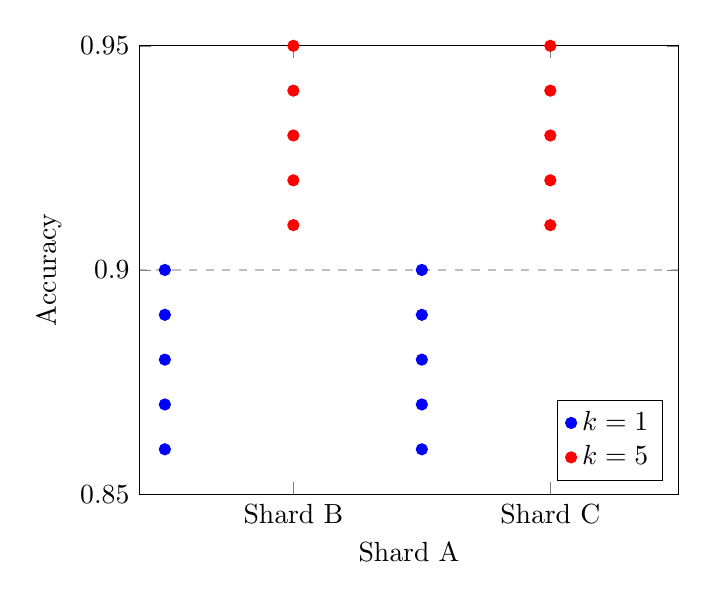
\begin{tikzpicture}
    \begin{axis}[
        xlabel={Shard A},
        ylabel={Accuracy},
        xmin=-0.2, xmax=4,
        ymin=0.85, ymax=0.95,
        xtick={1,3},
        xticklabels={Shard B, Shard C},
        ytick={0.85, 0.9, 0.95},
        legend pos=south east,
        ymajorgrids=true,
        grid style=dashed,
    ]

        % Data for Shard A - Top-1 Accuracy
        \addplot[
            color=blue,
            only marks,
            mark=*,
            mark options={solid},
        ] coordinates {
            (0, 0.86) (0, 0.87) (0, 0.88) (0, 0.89) (0, 0.90)
        };

        % Data for Shard A - Top-5 Accuracy
        \addplot[
            color=red,
            only marks,
            mark=*,
            mark options={solid},
        ] coordinates {
            (1, 0.91) (1, 0.92) (1, 0.93) (1, 0.94) (1, 0.95)
        };

        % Data for Shard B - Top-1 Accuracy
        \addplot[
            color=blue,
            only marks,
            mark=*,
            mark options={solid},
        ] coordinates {
            (2, 0.86) (2, 0.87) (2, 0.88) (2, 0.89) (2, 0.90)
        };

        % Data for Shard B - Top-5 Accuracy
        \addplot[
            color=red,
            only marks,
            mark=*,
            mark options={solid},
        ] coordinates {
            (3, 0.91) (3, 0.92) (3, 0.93) (3, 0.94) (3, 0.95)
        };

        \legend{$k = 1$, $k = 5$};

    \end{axis}
\end{tikzpicture}

\end{document}